% Autor: Simon May
% Datum: 2014-08-19

% XXX Ich finde, der Artikel sollte ein bisschen überarbeitet werden, der lässt uns so "unattraktiv" wirken ;-)
\section{Wenn das Fach schafft -- Fachschaft}
\begin{center}
\vspace{-0.5cm}

\includegraphics[width=0.7\textwidth]{res/fsphys_logo.pdf}
\vspace{-0.5cm}
\end{center}
\begin{multicols}{2}
% subsections in diesem Artikel kleiner (mit "\normalsize") darstellen,
% sonst ist zu wenig Platz
\addtokomafont{subsection}{\normalsize}
% etwas weniger Platz vor/nach subsections, sonst ist immer noch zu wenig Platz
\renewcommand{\fibelsubsectionpre}{\fibelsubsubsectionpre}
\renewcommand{\fibelsubsectionpost}{\fibelsubsubsectionpost}
\textbf{Wir schreiben das Jahr~2014. Die gesamte Studierendenschaft der Physik geht emsig und allein ihrem Studium nach.}

Alle?! Nein, nicht alle. Ein paar tapfere Studentinnen und Studenten leisten mutig dem allgemeinen Opportunismus Widerstand und engagieren sich in der Fachschaft. Neugierig? Aber was macht die Fachschaft eigentlich, möchtet ihr jetzt wahrscheinlich wissen. Das erste Mal kamst du wohl mit uns in Kontakt, als du dir überlegtest, an welcher Uni du wohl studieren möchtest. Wir haben versucht, dir ein wenig über das Physikstudium in Münster, die Wohnungssuche, die Stadt und ähnliches zu erzählen. Natürlich sind auch die Organisation und die Durchführung der Erstsemester-Orientierungseinheit (OE; "Ersti-Woche" bzw.\ "O-Woche") und des Ersti-Wochenendes Angelegenheiten der Fachschaft. Dies ist ein Teil unserer Bemühungen, die dir eine Hilfe am Studienanfang sein sollen.

\subsection*{Angebote zum Sonderpreis}
Zu unserem Angebot gehört aber auch das Verleihen von Alt-/Musterklausuren, Prüfungsprotokollen und Vorlesungsskripten\dots{} Das kann allerdings nur funktionieren, wenn mindestens einer aus eurem Semester auch Musterklausuren vorbeibringt und ihr Protokolle eurer Prüfungen zur Verfügung stellt, wenn es soweit ist. In Anbetracht der Tatsache, dass ihr dieses Angebot ja auch gerne und viel nutzen werdet, sollte das ja nicht zu viel verlangt sein -- ihr bekommt außerdem die Gewissheit, den nachfolgenden Generationen von Studenten in der "Schlacht" mit dem Physikstudium etwas weitergeholfen zu haben ;-)

\subsection*{Ersti-Arbeit, Ba-Ma-Tag und Evaluation}
Die Organisation der O-Woche liegt bei der Fachschaft, aber diese Arbeit kann sie nicht alleine machen, und so helfen immer einige Studenten aus verschiedenen Semestern mit, die sonst eigentlich wenig mit der Fachschaft zu tun haben. Meist sind das Studenten aus dem 3.~Semester. Auch, wenn es um das Ersti-Wochenende geht, ist diese Gruppe zur Stelle. Natürlich seid ihr aufgerufen, auch in den nächsten Semestern an dieser Ersti-Arbeit mitzuwirken.

\includegraphicscompressed[width=\columnwidth]{res/fsphys_foto_tafel.png}

Einmal im Jahr findet der sogenannte Ba-Ma-Tag statt. Das ist ein Tag, an dem sich die Arbeitsgruppen der Physik vorstellen. Arbeitsgruppen kann man auch mit Forschungsgruppen beschreiben, die durch einen Professor geleitet werden. Wenn ihr dann eure Bachelor- oder Masterarbeit schreiben wollt, so macht ihr das in diesen Gruppen. Deshalb soll allen Physikstudenten die Möglichkeit gegeben werden, einen Überblick über die verschieden Gebiete und Richtungen zu bekommen, um sich dann einer dieser Gruppen anzuschließen. Auch hier werden immer Personen gesucht, die mit organisieren und für das Drumherum sorgen.

Zweimal im Jahr, also jedes Semester, findet in allen Vorlesungen, Seminaren und Praktika eine Umfrage, Evaluation genannt, statt, die euch die Möglichkeit geben soll, dem Dozenten anonym Hinweise zu geben, was an seiner Veranstaltung gut ist oder noch verbessert werden kann. Auch diese Arbeit wird von der Fachschaft erledigt.

\subsection*{Sichtbare und unsichtbare Arbeit}
Ein großer Teil der Fachschaftsarbeit passiert für die normalen Studenten im Verborgenen. Dazu gehören fast alle Kommissionen und Gremien, in denen es auch studentische Vertreter gibt. Einige Beispiele auf Fachbereichs-Ebene:
\begin{description}
\item[FBR:] Der Fachbereichsrat, das höchste beschließende Gremium des Fachbereichs. Hierzu werden im Juni die studentischen Mitglieder per Briefwahl gewählt.
\item[KLSA:] Kommission für Lehre~\&~Studentische Angelegenheiten. Hier wird z.B.\ eine neue Prüfungs- und Studienordnung entwickelt.
\item[Berufungskommissionen:] Sie kümmern sich um die Neuberufung von Professoren und haben somit einen Einfluss darauf, welche Professoren an die Uni kommen.
\item[Prüfungskommissionen:] Kommissionen zu den verschiedenen Studiengängen, also Lehramt (2-Fach-Bachelor) und Bachelor bzw.\ Master (Physik und Geophysik).
\item[KFWN:] Kommission für Forschung~\&~wissenschaftlichen Nachwuchs.
\end{description}
In den meisten Fällen sind das auch Studenten aus der Fachschaft. Das muss aber eigentlich nicht so sein, und wenn ihr Lust habt, dann könnt ihr auch in einem solchen Gremium mitarbeiten. Ihr müsst euch dann nur melden und wir werden euch dann dafür vorschlagen.

Es gibt aber auch noch andere Arbeit um die sich die Fachschaft kümmert, so gibt es Anfang jeden Semesters eine große Physiker-Party, zu der ihr alle herzlich eingeladen seid. Diverse weitere Aktionen wie der Buchmarkt, das alljährliche Sommerfest und die Nikolaus-Aktion werden ebenfalls von uns organisiert. Ansonsten sind die Pinnwände vor den Fachschaftsräumen und die Homepage der Fachschaft immer ein Ort, an dem es neue Informationen rund um das Studium und das studentische Leben in Münster gibt.

\subsection*{Fachschaftssitzung}
Beschlussfassendes und vor allem diskutierendes Organ der Fachschaft ist die Fachschaftssitzung. Zurzeit findet die Sitzung mittwochs um 18~Uhr (s.t.~=~Punkt 18:00~Uhr) im Fachschaftsraum statt.
Jeder, der Lust hat, ist herzlich eingeladen, dort vorbeizukommen, denn die Fachschaft verhält sich aus Tradition streng basisdemokratisch und neue Gesichter beleben die Runde. Wer will, kann sich dann bei den Wahlen für die Fachschaftsvertretungen und das Studentenparlament, die immer im Wintersemester stattfinden, auch offiziell in die Fachschaft wählen lassen.

\fibelsig{Judith}
\begin{minipage}{\columnwidth}
	\begin{minipage}[t]{5cm}
	% Linksbündig und mit etwas Abstand zwischen Paragraphen
	\raggedright\parskip=0.1cm
	\textbf{Internetseite:}

	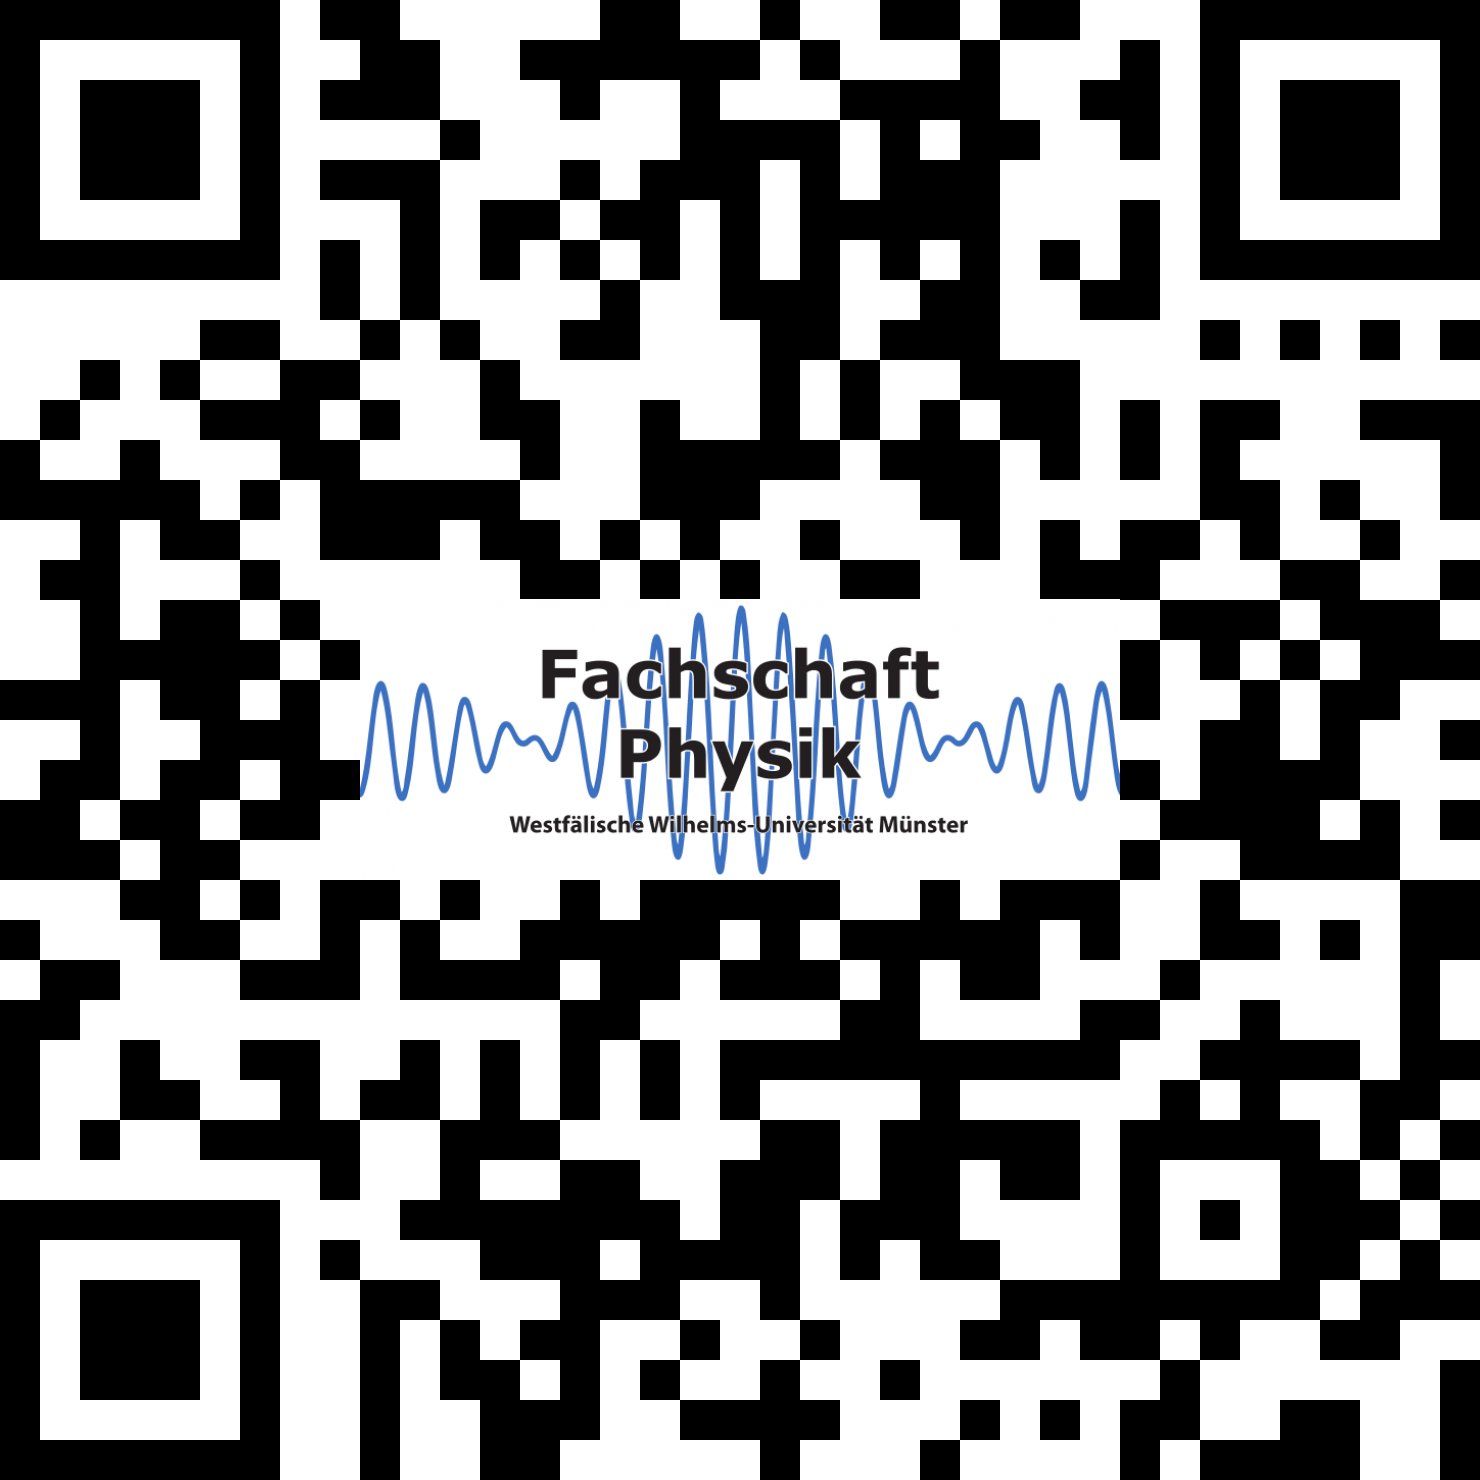
\includegraphics[width=3.8cm]{res/fsphys_qrcode_homepage.png}
	\scriptsize
	\href{https://www.uni-muenster.de/Physik.FSPHYS}{\texttt{fachschaft.physik.uni-muenster.de}}
	\end{minipage}
	\hfill
	\begin{minipage}[t]{4cm}
	% Rechtsbündig und mit etwas Abstand zwischen Paragraphen
	\raggedleft\parskip=0.1cm
	\textbf{Facebook-Seite:}

	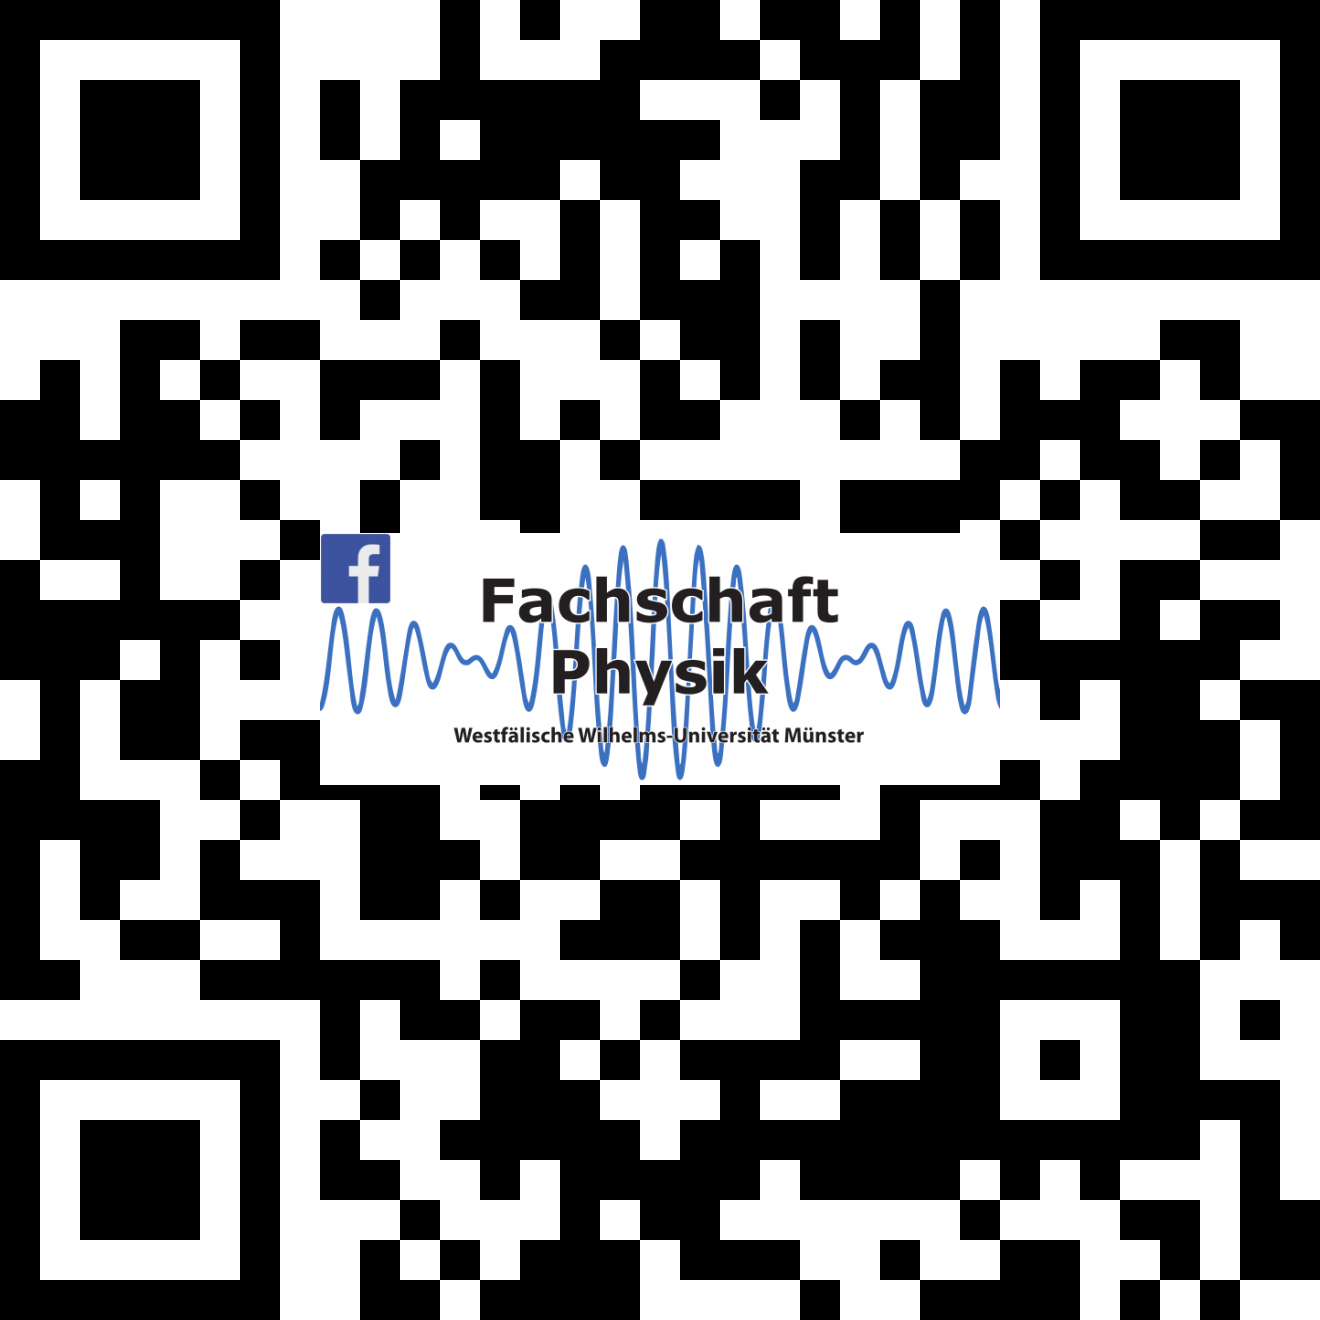
\includegraphics[width=3.8cm]{res/fsphys_qrcode_facebook.png}
	\scriptsize
	\href{https://facebook.com/fsphys}{\texttt{facebook.com/fsphys}}
	\end{minipage}
\end{minipage}
\end{multicols}
% Textbereich eine Seite größer machen, damit mehr Bild reinpasst
\enlargethispage{\baselineskip}
\begin{center}
\vspace{-0.4cm}
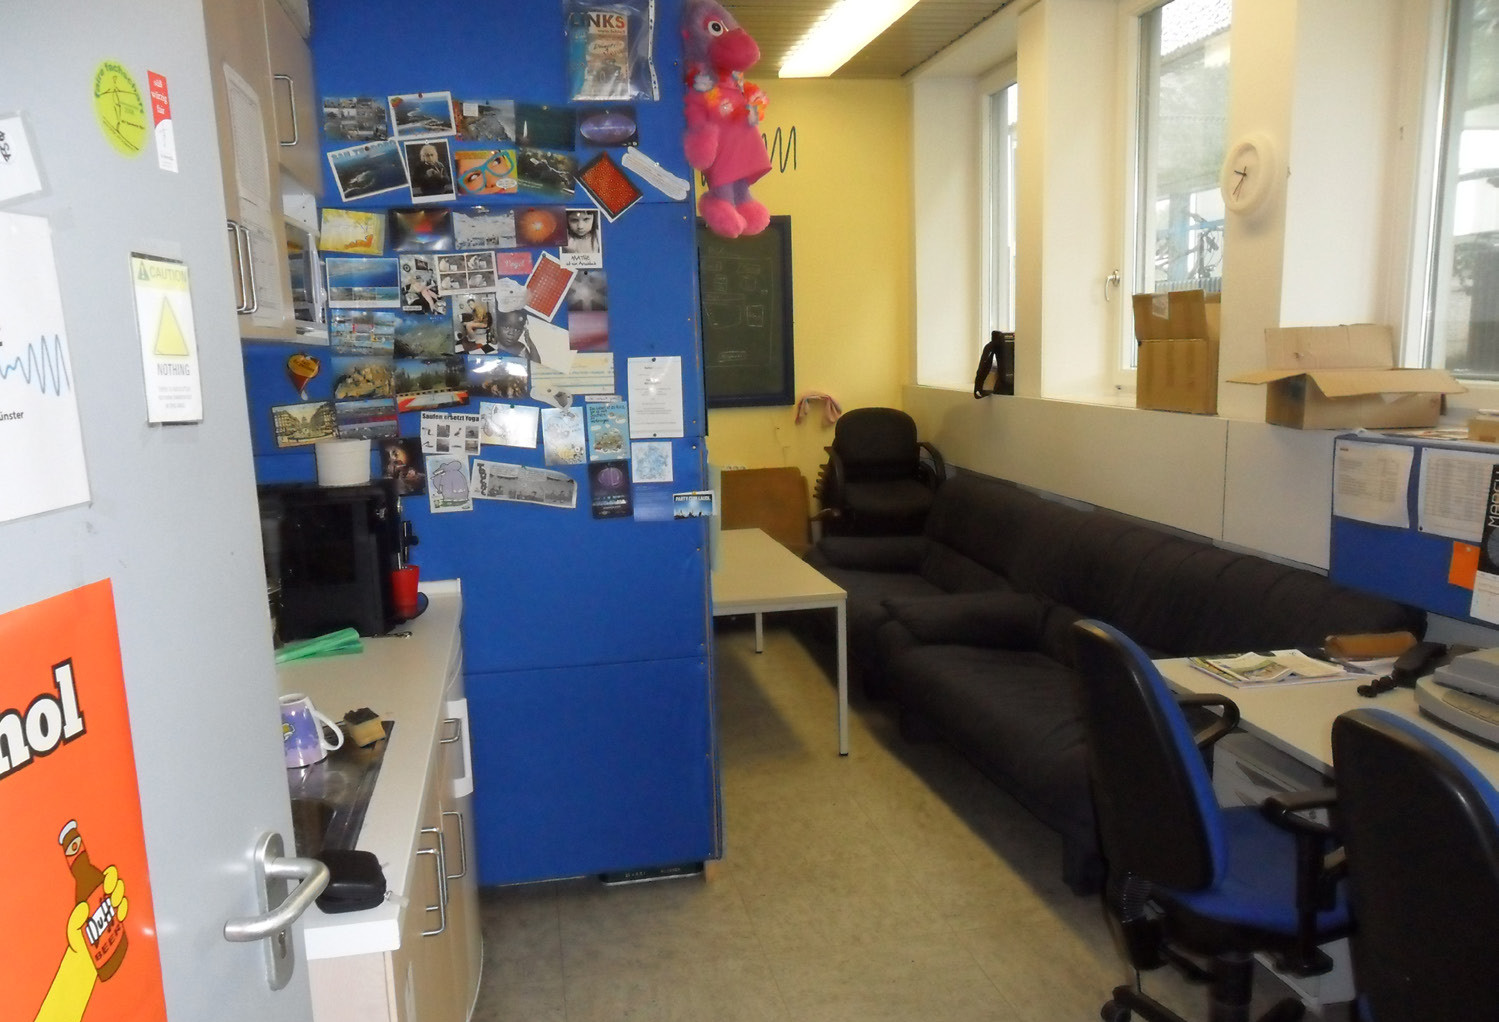
\includegraphics[width=0.7\textwidth]{res/fsphys_foto_fs_raum_cropped.jpg}
\end{center}


